\special{dvipdfmx:config z 0}
\documentclass{article}
\usepackage{marcythm}

\title{Undergraduate Complexity Theory \\ Lecture 12: NP-Completeness Reductions}
\author{Marcythm}
% \date{\today}
\date{July 15, 2022}

\begin{document}
\maketitle{}

\section{Lecture Notes}

Recap: poly-time mapping reduction \(\leq_m^P\), \( \prob{3COL} \leq_m^P \prob{4COL} \leq_m^P \prob{SAT} \leq_m^P \prob{CIRCUIT-SAT} \leq_m^P \prob{3SAT} \). Cook-Levin: \prob{CIRCUIT-SAT} is \NP-complete = \NP-hard + \NP.

Today: \(\prob{3SAT} \leq_m^P \prob{3COL}\) (which is hw5 p4), steps there to show
\begin{enumerate}
  \item \( \prob{3SAT} \leq_m^P \prob{E3SAT} \)
  \item \( \prob{3SAT} \leq_m^P \prob{NAE-3SAT} \)
  \item \( \prob{NAE-3SAT} \leq \prob{3COL} \)
\end{enumerate}

then show \(\prob{3COL} \leq_m^P \prob{INDEPENDENT-SET}\).

\begin{remark}
  Here all the 5 problems shown above are CSPs (Constraints Satisfaction Problem), but \prob{INDENPENDENT-SET} is not.
\end{remark}

To show \NP-completeness, given dicision problem \(L\),
\begin{enumerate}
  \item Show \(L \in \NP\) (usually easy)
  \item Pick \NP-hard \(S\) (e.g. \prob{3SAT}), show \(S \leq_m^P L\).
\end{enumerate}

\begin{definition}[\prob{E3SAT}]
  \prob{3SAT} with every clause having {\bf E}xactly 3 literals of distinct variables.
\end{definition}

\begin{theorem}
  \( \prob{3SAT} \leq_m^P \prob{E3SAT} \)
\end{theorem}

\begin{proof}
  Two cases to be considered:
  \begin{enumerate}
    \item In a clause there are two literal with the same variable, i.e. \(x \vee \neg x\). These clauses are always satisfied, so just remove them.
    \item In a clause there are only one or two literals. Add new variables \(a, b, c\) to \(\phi\), together with clauses \( (\neg a \vee b \vee c), (a \vee \neg b \vee c), (a \vee b \vee \neg c), (\neg a \vee \neg b \vee c), (\neg a \vee b \vee \neg c), (a \vee \neg b \vee \neg c), (\neg a \vee \neg b \vee \neg c) \), which restricts \(a = b = c = F\). Then add any of them into the clause to obtain the desired one.
  \end{enumerate}
\end{proof}

\begin{definition}[\prob{NAE-SAT}]
  same as \prob{CNF-SAT} \ul{except} instead requiring at least one true literal in each clause, we require that each clause has at least one literal assigned true and at least one literal assigned false. In other words, literals are {\bf N}ot {\bf A}ll {\bf E}qual to each other.
\end{definition}

\begin{theorem}
  \( \prob{3SAT} \leq_m^P \prob{NAE-3SAT} \)
\end{theorem}

\begin{proof}
  Prove this by showing \( \prob{3SAT} \leq_m^P \prob{s3SAT} \leq_m^P \prob{NAE-4SAT} \leq_m^P \prob{NAE-3SAT} \). (\hyperlink{https://math.stackexchange.com/questions/647710/how-do-i-reduce-3-sat-to-a-3-sat-nae-problem}{reference})

  First trivially convert \prob{3SAT} into the form where each clause contains exactly 3 terms (\prob{s3SAT}).

  The idea to show \( \prob{s3SAT} \leq_m^P \prob{NAE-4SAT} \): \( (a \vee b \vee c) \mapsto (a \vee b \vee c \vee s) \), where all clauses sharing the same \(s\). By symmetry, if \(s = {\it true}\) then at least one of \(a, b, c\) is false, just negate all the assignments can have \((a \vee b \vee c)\) satisfiable.

  The idea to show \( \prob{NAE-4SAT} \leq_m^P \prob{NAE-3SAT} \): \( (a \vee b \vee c \vee d) \mapsto (a \vee b \vee s) \wedge (\neg s \vee c \vee d) \).
\end{proof}

\begin{corollary}
  The proof above implies that \( \prob{E3SAT} \leq_m^P \prob{NAE-E3SAT} \).
\end{corollary}

\begin{remark}
  \prob{NAE-E3SAT} is convenient for further reductions, especially for problems with \ul{``symmetry''}.
\end{remark}

In \prob{NAE-SAT} there are no difference between T and F (which is not the case in \prob{3SAT}). Also in \prob{3COL} there are no difference between colors.

\begin{theorem}
  \( \prob{3SAT} \leq_m^P \prob{3COL} \)
\end{theorem}

\begin{proof}
  We do the proof in to steps.

  \begin{enumerate}
    \item Encode T/F assignment as a coloring. \\
    First fix a vertex, call it ``Ground''. By symmetry we WLOG assume it's colored Y. Then connect it with every pair of literals to form many triangles (which is also the NOT gate).
    % \begin{figure}[h]
    %   \centering
    %   \begin{tikzpicture}[every node/.style={draw=black, shape=circle}]
    %     \node (G) at (0, 0) {Ground};
    %     \node (x) at (-1, -1.73) {\(x\)};
    %     \node (negx) at (1, -1.73) {\(\neg x\)};

    %     \draw (G) -- (x);
    %     \draw (G) -- (negx);
    %     \draw (x) -- (negx);
    %   \end{tikzpicture}
    % \end{figure}

    \item Encode NAE constraints in \(G_{\phi}\). \\
    For each claus \(C\) in \(\phi\), add \ul{gadget}, subgraph that 3-colorable iff truth assignment induced by that 3-coloring satisfies \(C\).

    \begin{figure}[h]
      \centering
      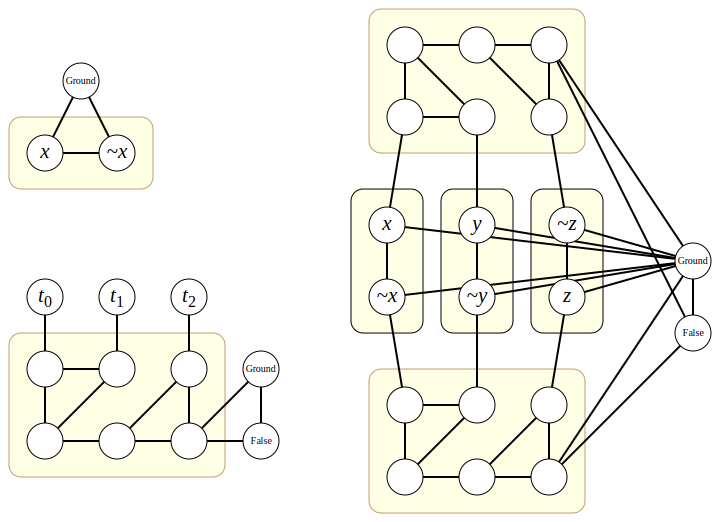
\includegraphics[width=0.8\textwidth]{assets/3SAT-3COL_reduction.pdf}
      \caption{construction of gadgets from wikipedia (gadget)}
    \end{figure}
  \end{enumerate}
\end{proof}

\begin{theorem}
  \( \prob{E3SAT} \leq_m^P \prob{INDENPENDENT-SET} \)
\end{theorem}

\begin{proof}
  Given \prob{E3SAT} instance \(\phi\), construct \(G_{\phi}, k_{\phi}\) s.t. \(\phi\) satisfiable iff \(G_{\phi}\) has a independent set of size \(k_{\phi}\). Roughly speaking,  one vertex for each literal in each clause (\(3n\) vertices in total, where \(n\) is \# of clauses), one edge for each pair of opposite literals (\(x\) and \(\neg x\)), and for each clause connect the three literals in it. Choose \(k_{\phi} = n\). We show the idea by an example.

  \begin{figure}
    \centering
    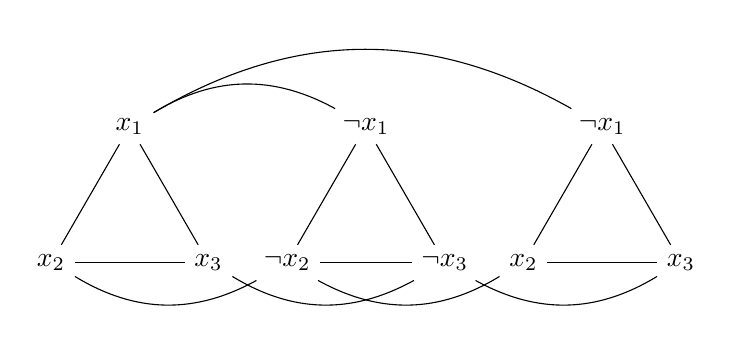
\begin{tikzpicture}
      \node (x1_1) at (-3, 0) {\(x_1\)};
      \node (nx1_1) at (0, 0) {\(\neg x_1\)};
      \node (nx1_2) at (3, 0) {\(\neg x_1\)};
      \node (x2_1) at (-4, -1.73) {\(x_2\)};
      \node (nx2_1) at (-1, -1.73) {\(\neg x_2\)};
      \node (x2_2) at (2, -1.73) {\(x_2\)};
      \node (x3_1) at (-2, -1.73) {\(x_3\)};
      \node (nx3_1) at (1, -1.73) {\(\neg x_3\)};
      \node (x3_2) at (4, -1.73) {\(x_3\)};

      \draw (x1_1) edge[bend left] (nx1_1);
      \draw (x1_1) edge[bend left] (nx1_2);
      \draw (x2_1) edge[bend right] (nx2_1);
      \draw (nx2_1) edge[bend right] (x2_2);
      \draw (x3_1) edge[bend right] (nx3_1);
      \draw (nx3_1) edge[bend right] (x3_2);

      \draw (x1_1) -- (x2_1);
      \draw (x2_1) -- (x3_1);
      \draw (x3_1) -- (x1_1);

      \draw (nx1_1) -- (nx2_1);
      \draw (nx2_1) -- (nx3_1);
      \draw (nx3_1) -- (nx1_1);

      \draw (nx1_2) -- (x2_2);
      \draw (x2_2) -- (x3_2);
      \draw (x3_2) -- (nx1_2);
    \end{tikzpicture}
    \caption{\(G_{\phi}\) for formula \((x_1 \vee x_2 \vee x_3) \wedge (\neg x_1 \vee \neg x_2 \vee \neg x_3) \wedge (\neg x_1 \vee x_2 \vee x_3)\), with \(k_{\phi} = 3\)}
  \end{figure}

  \newpage
  Intuitively, that is to choose one literal in each clause to be true, guaranteeing no two opposite literals are chosen at the same time.

  One thing should be noticed is that, cannot merge vertices for the same literal, since this would disable choosing one literal in multiple clause at the same time.
\end{proof}

\section{Reading}

\subsection{Sipser 7.5 (Additional \NP-complete Problems)}

\begin{enumerate}
  \item \prob{VERTEX-COVER} is \NP-complete, by showing \( \prob{3SAT} \leq_m^P \prob{VERTEX-COVER}. \)
  \item \prob{HAMPATH} is \NP-complete, by showing \( \prob{3SAT} \leq_m^P \prob{HAMPATH} \). \\
  remark: truth assignment corresponds to direction of path.
  \item \prob{UHAMPATH} is \NP-complete, by showing \( \prob{3SAT} \leq_m^P \prob{UHAMPATH} \), constructs from directed case.
  \item \prob{SUBSET-SUM} is \NP-complete, by showing \( \prob{3SAT} \leq_m^P \prob{SUBSET-SUM} \).
\end{enumerate}

\end{document}
